\documentclass{standalone}
\usepackage{tikz}
\usetikzlibrary{patterns, positioning}

\begin{document}
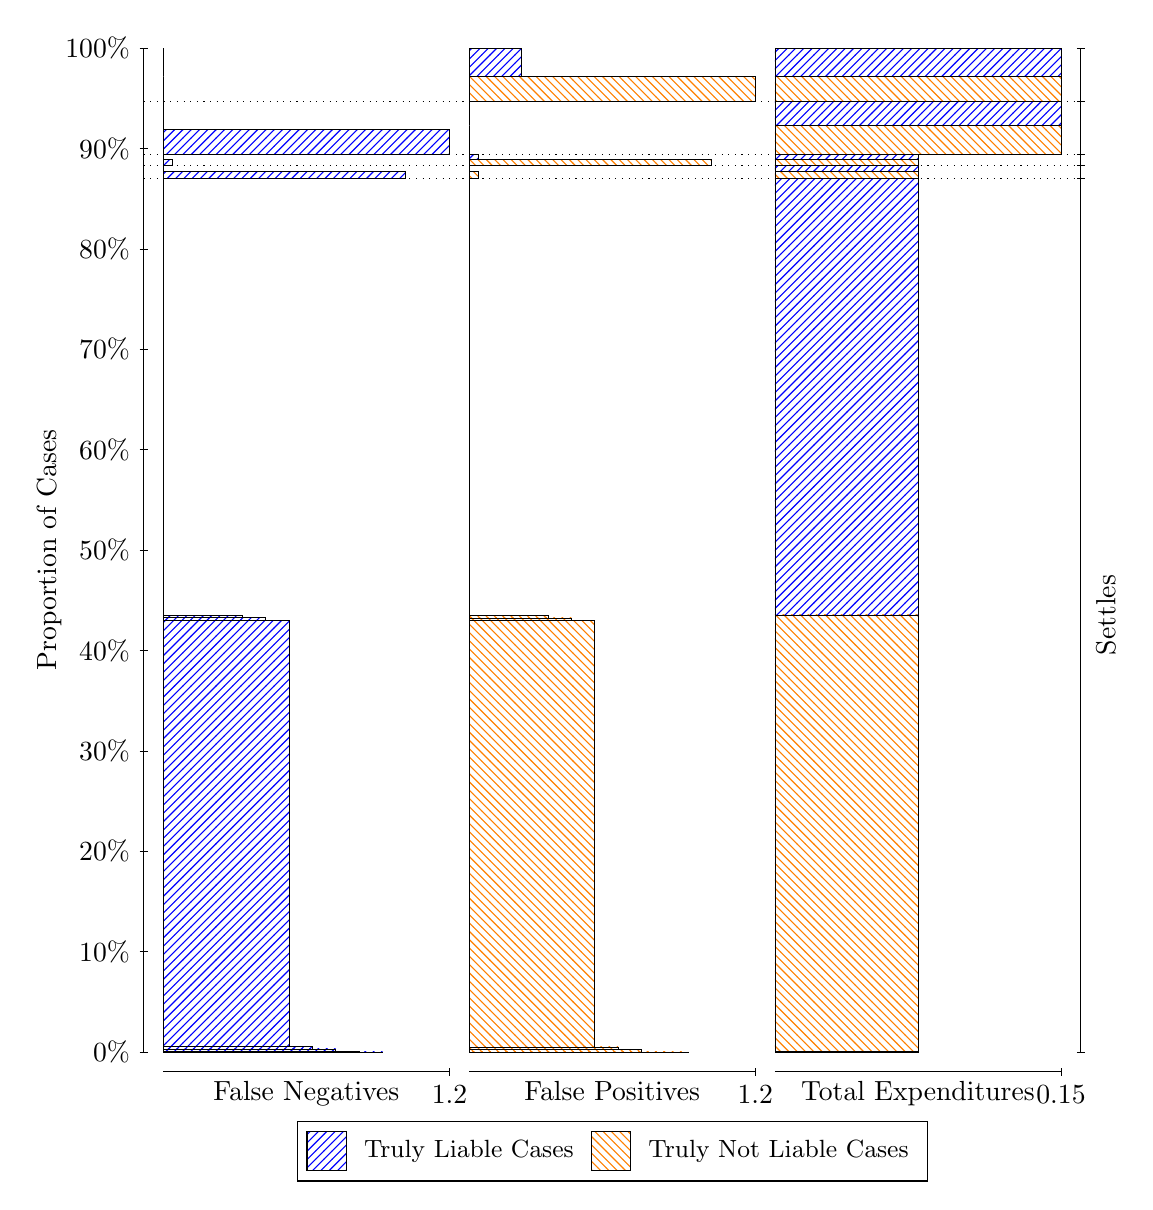
\begin{tikzpicture}
\draw[black, very thin] (1.5,1.75) -- (1.5,14.5);
\node[rotate=90, anchor=center] at (0.3, 8.125) {Proportion of Cases};
\draw[black, very thin] (1.45,1.75) -- (1.55,1.75);
\node[anchor=east] at (1.45, 1.75) {0\%};
\draw[black, very thin] (1.45,3.025) -- (1.55,3.025);
\node[anchor=east] at (1.45, 3.025) {10\%};
\draw[black, very thin] (1.45,4.3) -- (1.55,4.3);
\node[anchor=east] at (1.45, 4.3) {20\%};
\draw[black, very thin] (1.45,5.575) -- (1.55,5.575);
\node[anchor=east] at (1.45, 5.575) {30\%};
\draw[black, very thin] (1.45,6.85) -- (1.55,6.85);
\node[anchor=east] at (1.45, 6.85) {40\%};
\draw[black, very thin] (1.45,8.125) -- (1.55,8.125);
\node[anchor=east] at (1.45, 8.125) {50\%};
\draw[black, very thin] (1.45,9.4) -- (1.55,9.4);
\node[anchor=east] at (1.45, 9.4) {60\%};
\draw[black, very thin] (1.45,10.675) -- (1.55,10.675);
\node[anchor=east] at (1.45, 10.675) {70\%};
\draw[black, very thin] (1.45,11.95) -- (1.55,11.95);
\node[anchor=east] at (1.45, 11.95) {80\%};
\draw[black, very thin] (1.45,13.225) -- (1.55,13.225);
\node[anchor=east] at (1.45, 13.225) {90\%};
\draw[black, very thin] (1.45,14.5) -- (1.55,14.5);
\node[anchor=east] at (1.45, 14.5) {100\%};

\draw[black, very thin] (13.4,1.75) -- (13.4,14.5);
\draw[black, very thin] (13.35,1.75) -- (13.45,1.75);
\node[anchor=west] at (13.35, 1.75) {};
\draw[black, very thin] (13.35,12.847) -- (13.45,12.847);
\node[anchor=west] at (13.35, 12.847) {};
\draw[black, very thin] (13.35,13.013) -- (13.45,13.013);
\node[anchor=west] at (13.35, 13.013) {};
\draw[black, very thin] (13.35,13.152) -- (13.45,13.152);
\node[anchor=west] at (13.35, 13.152) {};
\draw[black, very thin] (13.35,13.826) -- (13.45,13.826);
\node[anchor=west] at (13.35, 13.826) {};
\draw[black, very thin] (13.35,14.5) -- (13.45,14.5);
\node[anchor=west] at (13.35, 14.5) {};

\draw[black, very thin, pattern color=blue, pattern=north east lines] (1.75,1.75) rectangle (4.5306,1.7525);
\draw[black, very thin, pattern color=blue, pattern=north east lines] (1.75,1.7525) rectangle (4.234,1.7527);
\draw[black, very thin, pattern color=blue, pattern=north east lines] (1.75,1.7527) rectangle (3.9374,1.7881);
\draw[black, very thin, pattern color=blue, pattern=north east lines] (1.75,1.7881) rectangle (3.6408,1.8239);
\draw[black, very thin, pattern color=blue, pattern=north east lines] (1.75,1.8239) rectangle (3.3442,7.2358);
\draw[black, very thin, pattern color=blue, pattern=north east lines] (1.75,7.2358) rectangle (3.0476,7.2659);
\draw[black, very thin, pattern color=blue, pattern=north east lines] (1.75,7.2659) rectangle (2.751,7.2966);
\draw[black, very thin, pattern color=blue, pattern=north east lines] (1.75,7.2966) rectangle (2.4544,7.2975);
\draw[black, very thin, pattern color=blue, pattern=north east lines] (1.75,7.2975) rectangle (2.1578,7.2987);
\draw[black, very thin, pattern color=orange, pattern=north west lines] (1.75,7.2987) rectangle (1.75,12.847);
\draw[black, very thin, pattern color=blue, pattern=north east lines] (1.75,12.847) rectangle (4.8272,12.931);
\draw[black, very thin, pattern color=orange, pattern=north west lines] (1.75,12.931) rectangle (1.75,13.013);
\draw[black, very thin, pattern color=blue, pattern=north east lines] (1.75,13.013) rectangle (1.8612,13.081);
\draw[black, very thin, pattern color=orange, pattern=north west lines] (1.75,13.081) rectangle (1.75,13.152);
\draw[black, very thin, pattern color=blue, pattern=north east lines] (1.75,13.152) rectangle (5.3833,13.462);
\draw[black, very thin, pattern color=orange, pattern=north west lines] (1.75,13.462) rectangle (1.75,13.826);
\draw[black, very thin, pattern color=orange, pattern=north west lines] (1.75,13.826) rectangle (1.75,14.136);
\draw[black, very thin, pattern color=blue, pattern=north east lines] (1.75,14.136) rectangle (1.75,14.5);
\draw[black, very thin, pattern color=orange, pattern=north west lines] (5.6333,1.75) rectangle (8.4139,1.7513);
\draw[black, very thin, pattern color=orange, pattern=north west lines] (5.6333,1.7513) rectangle (8.1173,1.7522);
\draw[black, very thin, pattern color=orange, pattern=north west lines] (5.6333,1.7522) rectangle (7.8207,1.784);
\draw[black, very thin, pattern color=orange, pattern=north west lines] (5.6333,1.784) rectangle (7.5241,1.8152);
\draw[black, very thin, pattern color=orange, pattern=north west lines] (5.6333,1.8152) rectangle (7.2276,7.2267);
\draw[black, very thin, pattern color=orange, pattern=north west lines] (5.6333,7.2267) rectangle (6.931,7.2613);
\draw[black, very thin, pattern color=orange, pattern=north west lines] (5.6333,7.2613) rectangle (6.931,7.2615);
\draw[black, very thin, pattern color=orange, pattern=north west lines] (5.6333,7.2615) rectangle (6.6344,7.296);
\draw[black, very thin, pattern color=orange, pattern=north west lines] (5.6333,7.296) rectangle (6.3378,7.2962);
\draw[black, very thin, pattern color=orange, pattern=north west lines] (5.6333,7.2962) rectangle (6.0412,7.2986);
\draw[black, very thin, pattern color=blue, pattern=north east lines] (5.6333,7.2986) rectangle (5.6333,12.847);
\draw[black, very thin, pattern color=orange, pattern=north west lines] (5.6333,12.847) rectangle (5.7446,12.929);
\draw[black, very thin, pattern color=blue, pattern=north east lines] (5.6333,12.929) rectangle (5.6333,13.013);
\draw[black, very thin, pattern color=orange, pattern=north west lines] (5.6333,13.013) rectangle (8.7105,13.084);
\draw[black, very thin, pattern color=blue, pattern=north east lines] (5.6333,13.084) rectangle (5.7446,13.152);
\draw[black, very thin, pattern color=orange, pattern=north west lines] (5.6333,13.152) rectangle (5.6333,13.517);
\draw[black, very thin, pattern color=blue, pattern=north east lines] (5.6333,13.517) rectangle (5.6333,13.826);
\draw[black, very thin, pattern color=orange, pattern=north west lines] (5.6333,13.826) rectangle (9.2667,14.136);
\draw[black, very thin, pattern color=blue, pattern=north east lines] (5.6333,14.136) rectangle (6.3007,14.5);
\draw[black, very thin, pattern color=orange, pattern=north west lines] (9.5167,1.75) rectangle (11.333,1.7526);
\draw[black, very thin, pattern color=blue, pattern=north east lines] (9.5167,1.7526) rectangle (11.333,1.7553);
\draw[black, very thin, pattern color=orange, pattern=north west lines] (9.5167,1.7553) rectangle (11.333,7.3013);
\draw[black, very thin, pattern color=blue, pattern=north east lines] (9.5167,7.3013) rectangle (11.333,12.847);
\draw[black, very thin, pattern color=orange, pattern=north west lines] (9.5167,12.847) rectangle (11.333,12.929);
\draw[black, very thin, pattern color=blue, pattern=north east lines] (9.5167,12.929) rectangle (11.333,13.013);
\draw[black, very thin, pattern color=orange, pattern=north west lines] (9.5167,13.013) rectangle (11.333,13.084);
\draw[black, very thin, pattern color=blue, pattern=north east lines] (9.5167,13.084) rectangle (11.333,13.152);
\draw[black, very thin, pattern color=orange, pattern=north west lines] (9.5167,13.152) rectangle (13.15,13.517);
\draw[black, very thin, pattern color=blue, pattern=north east lines] (9.5167,13.517) rectangle (13.15,13.826);
\draw[black, very thin, pattern color=orange, pattern=north west lines] (9.5167,13.826) rectangle (13.15,14.136);
\draw[black, very thin, pattern color=blue, pattern=north east lines] (9.5167,14.136) rectangle (13.15,14.5);
\draw[black, dotted] (1.5,12.847) -- (13.4,12.847);
\draw[black, dotted] (1.5,13.013) -- (13.4,13.013);
\draw[black, dotted] (1.5,13.152) -- (13.4,13.152);
\draw[black, dotted] (1.5,13.826) -- (13.4,13.826);
\draw[black, very thin] (1.75,1.5) -- (5.3833,1.5);
\node[anchor=north] at (3.5667, 1.5) {False Negatives};
\draw[black, very thin] (5.3833,1.45) -- (5.3833,1.55);
\node[anchor=north] at (5.3833, 1.45) {1.2};

\draw[black, very thin] (5.6333,1.5) -- (9.2667,1.5);
\node[anchor=north] at (7.45, 1.5) {False Positives};
\draw[black, very thin] (9.2667,1.45) -- (9.2667,1.55);
\node[anchor=north] at (9.2667, 1.45) {1.2};

\draw[black, very thin] (9.5167,1.5) -- (13.15,1.5);
\node[anchor=north] at (11.333, 1.5) {Total Expenditures};
\draw[black, very thin] (13.15,1.45) -- (13.15,1.55);
\node[anchor=north] at (13.15, 1.45) {0.15};

\node[black, centered, rotate=90] at (13.72, 7.2986) {Settles};





\draw (7.449999999999999,1.5) node[draw=none] (baseCoordinate) {};
\begin{scope}[align=center]
        \matrix[scale=0.5, draw=black, below=0.5cm of baseCoordinate, nodes={draw}, column sep=0.1cm]{
            \node[rectangle, draw, minimum width=0.5cm, minimum height=0.5cm, pattern=north east lines, pattern color=blue] {}; &
            \node[draw=none, font=\small] (B) {Truly Liable Cases}; &
            \node[rectangle, draw, minimum width=0.5cm, minimum height=0.5cm, pattern=north west lines, pattern color=orange] {}; &
            \node[draw=none, font=\small] (B) {Truly Not Liable Cases}; \\
            };
\end{scope}

\end{tikzpicture}
\end{document}